\documentclass[11pt]{article}
\usepackage{latexsym}
\usepackage{amsmath}
\usepackage{amssymb}
\usepackage{amsthm}
\usepackage{epsfig}
\usepackage[tight]{subfigure}
\usepackage{graphicx}
\graphicspath{ {./imgs/} }
\usepackage{amsmath}

\DeclareMathOperator*{\minimize}{min}
\DeclareMathOperator*{\maximize}{max}
\DeclareMathOperator*{\argmax}{arg\,max}
\DeclareMathOperator*{\argmin}{arg\,min}

\usepackage{algorithm}
 %on linux you may need to run sudo apt-get install texlive-full to install algorithm.sys
\usepackage{algorithmic}

\usepackage{verbatim}

\newcommand{\handout}[5]{
  \noindent
  \begin{center}
  \framebox{
    \vbox{
      \hbox to 5.78in { {#1} \hfill #2 }
      \vspace{4mm}
      \hbox to 5.78in { {\Large \hfill #5  \hfill} }
      \vspace{2mm}
      \hbox to 5.78in { {\em #3 \hfill #4} }
    }
  }
  \end{center}
  \vspace*{4mm}
}
\newcommand{\specialcell}[2][c]{%
  \begin{tabular}[#1]{@{}c@{}}#2\end{tabular}}
  
\newcommand{\lecture}[5]{\handout{#1}{#2}{#3}{#4}{#5}}
\newcommand{\collision}[0]{\mathrm{collision}}
\newcommand{\nocollision}[0]{\overline{\collision}}

\newcommand*{\QED}{\hfill\ensuremath{\square}}

\newtheorem{theorem}{Theorem}
\newtheorem{corollary}[theorem]{Corollary}
\newtheorem{lemma}[theorem]{Lemma}
\newtheorem{observation}[theorem]{Observation}
\newtheorem{proposition}[theorem]{Proposition}
\newtheorem{definition}[theorem]{Definition}
\newtheorem{claim}[theorem]{Claim}
\newtheorem{fact}[theorem]{Fact}
\newtheorem{assumption}[theorem]{Assumption}
\newtheorem{note}[theorem]{Note}

% 1-inch margins, from fullpage.sty by H.Partl, Version 2, Dec. 15, 1988.
\topmargin 0pt
\advance \topmargin by -\headheight
\advance \topmargin by -\headsep
\textheight 8.9in
\oddsidemargin 0pt
\evensidemargin \oddsidemargin
\marginparwidth 0.5in
\textwidth 6.5in

\parindent 0in
\parskip 1.5ex
%\renewcommand{\baselinestretch}{1.25}

\begin{document}

\lecture{Statistical Techniques in Robotics (16-831, S22)}{Lecture \#07
  (Wednesday, February 9)}{Lecturer: Kris Kitani}{Scribes: Jinkun Liu, Thomas Xu}{Follow the Regularized Leader}

\section{Review}
%This section serves as a review of the previous lecture and any other context required to frame the content of the current lecture. 

%You may format the scribes in any way you like, aside from changing font style, size and page format. Please use subsections and paragraphs to increase the readability of your notes.

%Length requirement 1-2 pages.

In the last lecture, we covered three main topics. First, the Winnow algorithm was discussed, which is an online linear classification algorithm. Second, online convex optimization was introduced, including the related concepts used to define an convex optimization problem. Finally, the Follow the Leader algorithm was introduced as a generic method for solving optimization problems.



%%%%%%%%%%%%%%%%%%%%%%%%%%%%%%%%
%%%%% winnow
%%%%%%%%%%%%%%%%%%%%%%%%%%%%%%%

\subsection{Winnow Algorithm}

The Winnow algorithm is an online linear classification algorithm that operates on binary features as inputs. The key assumption of the Winnow algorithm is that only a certain subset of the features are relevant for classification. Another key feature of Winnow algorithm is that it uses multiplicative weight updates, unlike the Perceptron algorithm which uses additive updates. Below is the pseudo code for this algorithm:

\begin{algorithm}[H]
\caption{Winnow algorithm}
\label{algo:winnow}
\begin{algorithmic}[1]
\STATE $\textbf{w}^{(1)} \leftarrow \{1,...,1\}$ \hfill $\triangleright$ Initialize weights
\FOR{$t=1,\;\cdots,\;T$}
\STATE \textsc{Receive} ($\textbf{x}^{(t)} \in\{0, 1\}^N$) \hfill $\triangleright$ Receive feature vector
\STATE $\hat{y}^{(t)} = \textbf{1}[\langle \textbf w^{(t)}, \textbf x^{(t)}\rangle>\Theta]$ \hfill $\triangleright$ Predict label
\STATE \textsc{Receive} ($y^{(t)}\in\{0, 1\}$) \hfill $\triangleright$ Receive true label
\STATE $w_n^{(t+1)}\leftarrow w_n^{(t)} (1+\beta)^{ (y^{(t)}-\hat{y}^{(t)})\cdot x_n^{(t)}} $ \hfill $\triangleright$ Update weights
\ENDFOR
\end{algorithmic}\label{algo:winnow}
\end{algorithm}
Here, $\Theta$ (often assumed equal to $N$) is the threshold that is used to define the decision boundary (hyperplane), and $\beta$ is a constant parameter that affects the magnitude of weight updates. A typical value is $\beta=1$. 
%From the expression in the exponential in the update rule (line 6), we can observe that weight updates are only performed when mistakes are made ($y^{(t)} \neq \hat{y}^{(t)}$), and only for weights corresponding to the positive input features ($x_n=1$). Additionally, the direction of weight updates depend on the type of mistakes (positive or negative) made.

Assuming $\beta=1$, the total number of mistakes $M$ made by the learner using the Winnow algorithm is upper-bounded as:
\begin{align}
    M<2+3k({\log_2 N+1})
\end{align}
where $N$ is the total number of input features and $k$ is the number of relevant features.

%%%%%%%%%%%%%%%%%%%%%%%%%%%%%%%%
%%%%% Online Convex Optimization
%%%%%%%%%%%%%%%%%%%%%%%%%%%%%%%
\subsection{Online Convex Optimization}
Online convex optimization serves as a generalized framework of many online tasks. In this framework, an online convex optimizer interacts with nature by producing predictions using its parameters $\boldsymbol{w}^{(t)}\in \mathcal{S}$, which are updated using the loss functions ${l}^{(t)}$ received from nature. Here, $\mathcal{S}$ must be a convex set and ${l}^{(t)}$ must be a convex function, both of which are defined below. 
\paragraph{Convex Set} A set $\mathcal{S}$ is considered a convex set if for all $\boldsymbol{w}, \boldsymbol{v} \in \mathcal{S}$:
\begin{align}
    \alpha \boldsymbol{w} + (1 - \alpha) \boldsymbol{v} \in \mathcal{S} \quad \quad \forall \alpha \in [0,1]
\end{align}
% In other words, the points that lie linearly between $\boldsymbol{w}$ and $\boldsymbol{v}$ must all also be inside $\mathcal{S}$. The $\alpha$ term indicates how far along a given point is between $\boldsymbol{w}$ and $\boldsymbol{v}$.
\paragraph{Convex Function}
A function $f : \mathcal{S} \rightarrow \mathbb{R}$ is considered a convex function if for all $\boldsymbol{w}, \boldsymbol{v} \in \mathcal{S}$:
\begin{align}
    f(\alpha \boldsymbol{w} + (1 - \alpha) \boldsymbol{v}) \leq \alpha f(\boldsymbol{w}) + (1 - \alpha) f(\boldsymbol{v}) \quad \quad \forall \alpha \in [0,1]
    \label{eqn:convex_func}
\end{align}
% The interpretation of this definition is as follows: the right-hand side of the inequality forms a straight line between two points $f(\boldsymbol{w})$ and $f(\boldsymbol{v})$. All points on this line must be above or equal to the function itself across the same interval, for the function to be convex.
\paragraph{Lipschitz Continuity}
A function $f(\cdot)$ is ``L-Lipschitz" over set $\mathcal{S}$ with respect to a norm $\Vert \cdot \Vert$ if:
\begin{equation}
    \label{eq:lipschitz}
    |f(\boldsymbol{u}) - f(\boldsymbol{w})| \leq L || \boldsymbol{u} - \boldsymbol{w} || \quad \quad \forall \boldsymbol{u}, \boldsymbol{w} \in \mathcal{S}
\end{equation}
% Here, $L$ is the ``Lipschitz constant." This expression essentially sets a bound on the function’s rate of change. 
For a problem to be solved with convex optimization, the function and solution space must both be convex; in addition, the function must be either convex-Lipschitz-bounded or convex-smooth-bounded.
\paragraph{Convexification}
Non-convex problems can be converted into convex ones. One method is convexification by \textbf{randomization}, such as in the case of converting WMA to RWMA. Another method is convexification by \textbf{surrogate loss}, which replaces the original non-convex loss function with a surrogate loss function that upper-bounds the original loss function, and is itself a convex function.
%%%%%%%%%%%%%%%%%%%%%%%%%%%%%%%%
%%%%% Follow the Leader (review)
%%%%%%%%%%%%%%%%%%%%%%%%%%%%%%%
\subsection{Follow the Leader}
Follow the Leader (FTL) is a generic algorithm for online (not necessarily convex) optimization problems. Its main idea is that the learner should go by the best choice seen so far. The general pseudocode for FTL is as seen below:
\begin{algorithm}[H]
\caption{Follow the Leader}
\label{algo:FTL}
\begin{algorithmic}[1]
\FOR{$t=1,2,\;\cdots,\;T$}
\vspace{5pt}
\STATE \qquad  $\boldsymbol{w}^{(t)}=\text{arg min}_{\boldsymbol{w}\in W} \sum_{i=1}^{t-1} f^{(i)} (\boldsymbol{w})$
\vspace{5pt} \hfill $\triangleright$ Update parameter
\STATE \qquad  $\textsc{Receive}(f^{(t)}:W \rightarrow \mathbb{R})$ \hfill $\triangleright$ Receive loss
\ENDFOR
\end{algorithmic}
\end{algorithm}
The performance of FTL is affected by the loss function used. Note that $W$ is a convex set. With a linear loss of the form $f^{(t)} = \boldsymbol{w} \cdot \boldsymbol{z}^{(t)}$, $O(T)$ loss and regret is possible in an adversarial scenario; the quadratic loss $f^{(t)}=\frac{1}{2}\Vert \boldsymbol{w}-\boldsymbol{z}^{(t)}\Vert^2_2$ can achieve $O(\sqrt{T})$ regret, as we will derive in the main summary. 
\section{Summary}
%%%%%%%%%%%%%%%%%%%%%%%%%%%%%%%%
%%%%% FTL regret bound
%%%%%%%%%%%%%%%%%%%%%%%%%%%%%%%
\subsection{Follow the Leader Regret Bound}
\label{sec:FTL}
To derive the generic FTL's regret bound (without any assumptions on the form of the loss function), we upper-bound the regret using the technique \textbf{one-step look ahead cheater}. The regret of FTL is of the form:
\begin{align}
    R(\boldsymbol{u})=\sum_t [f^{(t)}(\boldsymbol{w}^{(t)})-f^{(t)}(\boldsymbol{u})]
\end{align}
where $\boldsymbol{u}$ is any set of parameters, $\boldsymbol{w}^{(t)}$ is learner's set of parameters at time $t$, and $f^{(t)}$ is the loss function returned by nature. We can upper-bound the performance of $\boldsymbol{u}$ by setting it to a one-step look ahead cheater that has access to the loss function at time $t$, $\boldsymbol{w}^{(t+1)}$:
\begin{align}
\label{eq:propose}
    \sum_t [f^{(t)}(\boldsymbol{w}^{(t)})-f^{(t)}(\boldsymbol{u})] \leq \sum_{t}[f^{(t)}(\boldsymbol{w}^{(t)}) - f^{(t)}(\boldsymbol{w}^{(t+1)})]
\end{align}
Subtracting $f^{(t)}(\boldsymbol{w}^{(t)})$ from both sides, we get:
\begin{align}
     \sum_{t=1}^T f^{(t)}(\boldsymbol{w}^{(t+1)}) \leq     \sum_{t=1}^T f^{(t)}(\boldsymbol{u})\;\;\;\;\; \forall \boldsymbol{u}
         \label{eq:cheater}
\end{align}
This relationship indicates that the loss of a series of one-step look ahead cheaters is equal to or smaller than the loss of any other set of parameters $\boldsymbol{u}$. To prove (\ref{eq:cheater}), we use proof by induction and assume it's true for $T-1$, and will prove that it holds true for $T$:
\begin{align}
\label{eq:assume}
     \sum_{t=1}^{T-1} f^{(t)}(\boldsymbol{w}^{(t+1)}) \leq     \sum_{t=1}^{T-1} f^{(t)}(\boldsymbol{u})
\end{align}
Adding $f^{(t)}(\boldsymbol{w}^{(T+1)})$, the loss of the one-step look ahead cheater for the next time step, to both sides:
\begin{align}
\label{eq:addbothside}
    \sum_{t=1}^{T} f^{(t)} (\boldsymbol{w}^{(t+1)})\leq f^{(T)}(\boldsymbol{w}^{(T+1)}) +  \sum_{t=1}^{T-1} f^{(t)} (\boldsymbol{u})
\end{align}
Note that the added term has been collapsed into the summation on the left side of \ref{eq:addbothside}, but not on the right side due the different parameters. However, since we assume that (\ref{eq:assume}) and by extension (\ref{eq:addbothside}) is true for all $\boldsymbol{u}$, we can simply substitute $\boldsymbol{u}=\boldsymbol{w}^{(T+1)}$:
\begin{align}
\label{eq:bigsmallt}
    \sum_{t=1}^{T} f^{(t)} (\boldsymbol{w}^{(t+1)})&\leq\sum_{t=1}^{T} f^{(t)} (\boldsymbol{w}^{(T+1)})
\end{align}
In (\ref{eq:bigsmallt}), the left side is the loss for always using the one-step look ahead cheater, and the right side is the loss for using the single cheater at the end of the sequence for all time steps. Recall the definition of the minimizer: $\boldsymbol{w}^{(T+1)} = \text{argmin}_{\boldsymbol{u} \in S} \sum_{t=1}^T f^{(t)}(\boldsymbol{u})$. This allows us to upper-bound the right hand side of (\ref{eq:bigsmallt}) by all $\boldsymbol{u}$:
\begin{align}
           \sum_{t=1}^{T} f^{(t)} (\boldsymbol{w}^{(t+1)})
       \leq \sum_{t=1}^{T} f^{(t)} (\boldsymbol{u})
\end{align}
Multiply both sides by -1 and add $f^{(t)}(\boldsymbol{w}^{(t)})$ to the summation on both sides, we finally obtain the regret bound of the generic FTL algorithm proposed in (\ref{eq:propose}):
\begin{align}
        R(\boldsymbol{u})&=\sum_t [f^{(t)}(\boldsymbol{w}^{(t)})-f^{(t)}(\boldsymbol{u})]\\
        &\leq \sum_t [f^{(t)}(\boldsymbol{w}^{(t)})-f^{(t)} (\boldsymbol{w}^{(t+1)})]
\label{eq:FTLregret}
\end{align}

%%%%%%%%%%%%%%%%%%%%%%%%%%%%%%
% FTL quadratic
%%%%%%%%%%%%%%%%%%%%%%%%%%%%%%%
\subsubsection{Follow the Leader (Quadratic Loss) Regret Bound}
To derive the regret bound for FTL with quadratic loss, we simply substitute the specific quadratic loss function into the generic regret bound derived for generic FTL above (\ref{eq:FTLregret}). Note that we assume points $\boldsymbol{z}$ are bounded such that $||\boldsymbol{z}||^2_2 \leq L$. Recall that the quadratic loss is given by:
\begin{align}
    f^{(t)}(\boldsymbol{w})=\frac{1}{2}\Vert \boldsymbol{w}-\boldsymbol{z}^{(t)}\Vert^2_2
\end{align}
This leads to the following expression for a single time step:
\begin{align}
    f^{(t)}(\boldsymbol{w}^{(t)}) - f^{(t)}(\boldsymbol{w}^{(t+1)}) = \frac{1}{2}||\boldsymbol{w}^{(t)} - \boldsymbol{z}^{(t)}||_2^2 - \frac{1}{2}||\boldsymbol{w}^{(t+1)} - \boldsymbol{z}^{(t)}||_2^2
    \label{eq:FTL_quad_initial}
\end{align}
Additionally, recall that the minimizer of this quadratic loss is simply the mean:
\begin{align}
    \boldsymbol{w}^{(t)} = \frac{1}{t-1}\sum_{i=1}^{t-1} {\boldsymbol{z}}^{(i)}
    \label{eq:FTL_avg_z}
\end{align}
Knowing this, we can rewrite the weight update at each time step in an incremental form:
\begin{align}
    \boldsymbol{w}^{(t+1)} = (1-\frac{1}{t})\boldsymbol{w}^{(t)} + (\frac{1}{t})\boldsymbol{z}^{(t)}
\end{align}
Substituting this incremental form into (\ref{eq:FTL_quad_initial}) and rearranging yields:
\begin{align}
    f^{(t)}(\boldsymbol{w}^{(t)}) - f^{(t)}(\boldsymbol{w}^{(t+1)}) &= \frac{1}{2}||\boldsymbol{w}^{(t)} - \boldsymbol{z}^{(t)}||_2^2 - \frac{1}{2}||(1-\frac{1}{t})\boldsymbol{w}^{(t)} + (\frac{1}{t})\boldsymbol{z}^{(t)} - \boldsymbol{z}^{(t)}||_2^2\\
    &=\frac{1}{2} \Big( 1- \big( 1-\frac{1}{t} \big) ^2 \Big) ||\boldsymbol{w}^{(t)} - \boldsymbol{z}^{(t)}||_2^2
    \label{eq:FTL_quad_middle})
\end{align}
Note that the $(1-\frac{1}{t})$ term becomes squared after it is factored out of the squared L2 norm. Next, we make use of the following known inequality (illustrated in Figure \ref{fig:known}):
\begin{align}
    \frac{1}{2} \Big( 1- \big( 1-\frac{1}{t} \big) ^2 \Big) \leq \frac{1}{t}
    \label{eq:known}
\end{align}
\begin{figure}[h]
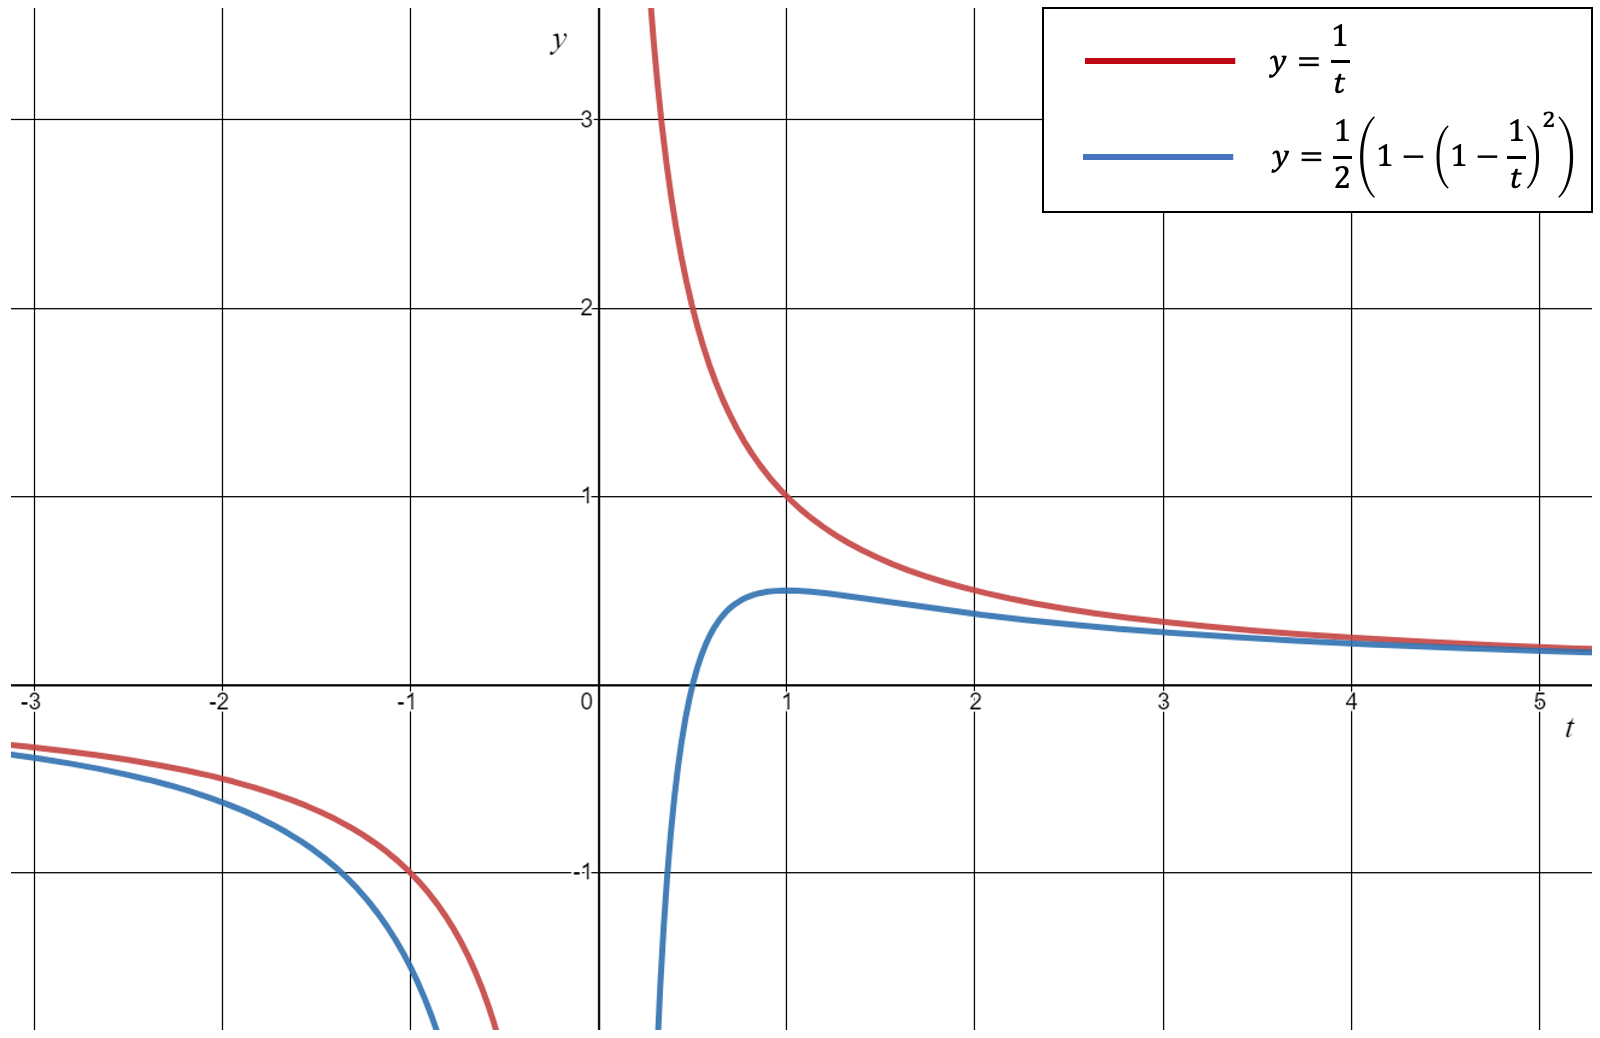
\includegraphics[scale=0.5]{imgs/known.png}
\centering
\caption{The known inequality used in (\ref{eq:known}).}
\label{fig:known}
\end{figure}

Applying this known inequality to (\ref{eq:FTL_quad_middle}) yields:
\begin{align}
    f^{(t)}(\boldsymbol{w}^{(t)}) - f^{(t)}(\boldsymbol{w}^{(t+1)}) \leq \Big( \frac{1}{t} \Big) ||\boldsymbol{w}^{(t)} - \boldsymbol{z}^{(t)}||_2^2
    \label{eq:FTL_quad_end}
\end{align}

Next, we make use of the following assumptions:
\begin{enumerate}
    \item $L = \max_t ||\boldsymbol{z}^{(t)}||$
    \item $||\boldsymbol{w}^{(t)}|| \leq L$
    \item $||\boldsymbol{w}^{(t)} - \boldsymbol{z}^{(t)}|| \leq 2L$
\end{enumerate}

The first assumption states that $L$ is a constant value and comes from our earlier assumption that each point $z$ is bounded. The second assumption states that the average value of the points (see (\ref{eq:FTL_avg_z})) is less than or equal to the max value of the individual points. The third assumption results from the first two; $w^{(t)}$ and $z^{(t)}$ can be thought of as two vectors with max length $L$, and from the triangle inequality, the line that connects their ends can have max length $2L$.

Applying these assumptions yields the following regret bound for a single time step:
\begin{align}
    f^{(t)}(\boldsymbol{w}^{(t)}) - f^{(t)}(\boldsymbol{w}^{(t+1)}) \leq \Big( \frac{1}{t} \Big) 4L^2
    \label{eq:FTL_quad_regret_single}
\end{align}
To obtain the regret bound over all time steps, we substitute (\ref{eq:FTL_quad_regret_single}) into (\ref{eq:FTLregret}):
\begin{align}
    R(\boldsymbol{u}) \leq \sum_t [f^{(t)}(\boldsymbol{w}^{(t)})-f^{(t)} (\boldsymbol{w}^{(t+1)})] \leq 4L^2\sum_t (\frac{1}{t})
    \label{eq:total_regret_ineq}
\end{align}
Additionally, we make use of the following known inequality:
\begin{align}
    \sum_{t=1}^T(\frac{1}{t}) \leq 1 + \int_1^T (\frac{1}{t}) dt = \text{log}(T) + 1
    \label{eq:riemann_ineq}
\end{align}
Combining (\ref{eq:FTL_quad_regret_single}), (\ref{eq:total_regret_ineq}), and (\ref{eq:riemann_ineq}) yields the final expression for the regret bound for FTL with quadratic loss:
\begin{align}
    \text{Regret} \leq 4L^2 \Big( \text{log}(T) + 1 \Big)
\end{align}
Note that this grows sub-linearly in time ($O(\text{log}(T))$), making FTL with quadratic loss a no-regret algorithm. Another observation for quadratic loss is that since the weight updates are done via averaging, the weights do not change drastically in one time step; this ensures smoother weight udpates and the stability of the algorithm.

\normalfont

%%%%%%%%%%%%%%%%%%%%%%%%%%%%%%%%
%%%%% FTRL
%%%%%%%%%%%%%%%%%%%%%%%%%%%%%%%

\subsection{Follow the Regularized Leader}
Compared to FTL, Follow the Regularized Leader (FTRL) adds an explicit regularization term $\psi$ to the parameter update step. One benefit of the regularization is that it improves the stability of the chosen parameters $\boldsymbol{w}$ ($\boldsymbol{w}\in S$ where $S$ is a convex set).

The generic algorithm for FTRL is shown below.

\begin{algorithm}[H]
\caption{Follow the Regularized Leader}
\label{algo:FTRL}
\begin{algorithmic}[1]
\FOR{$t=1,2,\;\cdots,\;T$}
\vspace{5pt}
\STATE \qquad  $\boldsymbol{w}^{(t)}=\text{arg min}_{\boldsymbol{w}\in S} \sum_{i=1}^{t-1} f^{(i)} (\boldsymbol{w}) + \psi (\boldsymbol{w})$
\vspace{5pt} \hfill $\triangleright$ Update parameter with regularization
\STATE \qquad  $\textsc{Receive}(f^{(t)}:S \rightarrow \mathbb{R})$ \hfill $\triangleright$ Receive loss
\ENDFOR
\end{algorithmic}
\end{algorithm}

Here, $\psi (\boldsymbol{w})$ represents the regularization term, and is a scalar-valued function: $\psi : S \rightarrow \mathbb{R}$. FTL can be seen as a special case of FTRL where $\psi=0$. 

We will use this observation to derive FTRL's \textbf{regret bound} using the already derived FTL regret bound. In particular, we can treat the regularization term $\psi (\boldsymbol{w})$ as the loss function $f^{(0)} (\boldsymbol{w})$ at $t=0$. This is because at $t=0$, no loss function has been received from nature, so the minimizer will set $\boldsymbol{w}$ to the value that minimizes $\psi (\boldsymbol{w})$ only: 
\begin{align}
    \boldsymbol{w}^{(t)}&=\text{arg min}_{\boldsymbol{w}\in S} \sum_{i=1}^{t-1} f^{(i)} (\boldsymbol{w}) + \psi (\boldsymbol{w})\\
    &=\text{arg min}_{\boldsymbol{w}\in S} \sum_{i=1}^{t-1} f^{(i)} (\boldsymbol{w}) + f^{(0)} (\boldsymbol{w})
\end{align}
Recall the regret bound for generic FTL from (\ref{eq:FTLregret}):
\begin{align}
        R(\boldsymbol{u})=\sum_t [f^{(t)}(\boldsymbol{w}^{(t)})-f^{(t)}(\boldsymbol{u})]
        \leq \sum_t [f^{(t)}(\boldsymbol{w}^{(t)})-f^{(t)} (\boldsymbol{w}^{(t+1)})]
\end{align}
Add the loss function $f^{(0)}$ at $t=0$ to both sides:
\begin{align}
        [f^{(0)} (\boldsymbol{w}^{(0)})-f^{(0)} (\boldsymbol{u})]&+\sum_{i=1}^{T} [f^{(t)}(\boldsymbol{w}^{(t)})-f^{(t)}(\boldsymbol{u})]\\
        &\leq [f^{(0)} (\boldsymbol{w}^{(0)})-f^{(0)} (\boldsymbol{w}^{(1)})]+\sum_{i=1}^{T} [f^{(t)}(\boldsymbol{w}^{(t)})-f^{(t)} (\boldsymbol{w}^{(t+1)})]
\end{align}
Substitute $f^{(0)}$ with $\psi$, which is essentially a change in notation:
\begin{align}
        [\psi (\boldsymbol{w}^{(0)})-\psi (\boldsymbol{u})]&+\sum_{i=1}^{T} [f^{(t)}(\boldsymbol{w}^{(t)})-f^{(t)}(\boldsymbol{u})]\\
        &\leq [\psi (\boldsymbol{w}^{(0)})-\psi (\boldsymbol{w}^{(1)})]+\sum_{i=1}^{T} [f^{(t)}(\boldsymbol{w}^{(t)})-f^{(t)} (\boldsymbol{w}^{(t+1)})]
\end{align}
Subtract $[\psi (\boldsymbol{w}^{(0)})-\psi (\boldsymbol{u})]$ from both sides yields the regret bound for the generic FTRL algorithm:
\begin{align}
    R(\boldsymbol{u}) \leq \Big[ \psi(\boldsymbol{u}) - \psi(\boldsymbol{w}^{(1)} \Big] + \sum_{t=1}^T \Big[ f^{(t)}(\boldsymbol{w}^{(t)}) - f^{(t)}(\boldsymbol{w}^{(t+1)})\Big]
    \label{eq:FTRL_generic_regret}
\end{align}
This regret bound will be used as a intermediate step for the derivation of regret bound of FTRL with linear loss and quadratic regularization.

%%%%%%%%%%%%%%%%%%%%%%%%%%%%%%%
% FTRL with Linear loss and quad reg
%%%%%%%%%%%%%%%%%%%%%%%%%%%%%%%%%%%%%
\subsubsection{FTRL with Linear Loss Function and Quadratic Regularization}
For this section, let us consider a linear loss function of the form $f^{(t)} = \boldsymbol{w} \cdot \boldsymbol{z}^{(t)}$. Recall from last lecture that the unregularized FTL with linear loss has unstable weight updates and $O(T)$ regret. Next, we add in quadratic regularization:
\begin{align}
    \psi(\boldsymbol{w}) = \frac{1}{2\eta}||\boldsymbol{w}||_2^2
\end{align}
Note that this regularization function penalizes large values and tries to ``pull" parameters towards zero. This new term changes the FTRL learner prediction rule to:
\begin{align}
    \boldsymbol{w}^{(t)} = \argmin_{\boldsymbol{w} \in S} \Big( \frac{1}{2\eta}||\boldsymbol{w}||^2_2 + \boldsymbol{w} \cdot \sum_{i=1}^{t-1} \boldsymbol{z}^{(i)} \Big)
    \label{eq:FTRL_quad_reg_pred_rule}
\end{align}
To solve the minimizer, take the derivative of the cumulative loss (the expression within the parentheses in (\ref{eq:FTRL_quad_reg_pred_rule})) with respect to $\boldsymbol{w}$ and set equal to zero to obtain:
\begin{align}
    \frac{2\boldsymbol{w}}{2\eta} + \sum_{i=1}^{t-1}\boldsymbol{z}^{(i)}=0
\end{align}
\begin{align}
    \boldsymbol{w}^{(t)} = -\eta \sum_{i=1}^{t-1}\boldsymbol{z}^{(i)}
\end{align}
Note that the shorthand $\theta^{(t)}=\sum_{i=1}^{t-1}\boldsymbol{z}^{(i)}$ is often used.

We can also decompose the equation for the minimizer into a recursive form:
\begin{align}
    &\boldsymbol{w}^{(t)} = -\eta \sum_{i=1}^{t-1}\boldsymbol{z}^{(i)} \\
    \implies &\boldsymbol{w}^{(t)} = -\eta \Big( \sum_{i=1}^{t-2}\boldsymbol{z}^{(i)}  + \boldsymbol{z}^{(t-1)} \Big) \\
    \implies &\boldsymbol{w}^{(t)} = -\eta \sum_{i=1}^{t-2}\boldsymbol{z}^{(i)} - \eta \boldsymbol{z}^{(t-1)} \\
    \implies &\boldsymbol{w}^{(t)} = \boldsymbol{w}^{(t-1)} -\eta \boldsymbol{z}^{(t-1)}
    \label{eq:FTRLupdate}
\end{align}
(\ref{eq:FTRLupdate}) is an update equation that allows us to update $\boldsymbol{w}$ incrementally at each time step. Furthermore, we can see that the update term $-\eta \boldsymbol{z}^{(t-1)}$ is proportional to $\boldsymbol{z}^{(t-1)}$, the gradient of the loss function $f^{(t)} = \boldsymbol{w} \cdot \boldsymbol{z}^{(t)}$ at $t-1$.

To derive the \textbf{regret bound} for this FTRL variant, substitute the linear loss function and quadratic regularization function into the generic FTRL regret bound (\ref{eq:FTRL_generic_regret}):
\begin{align}
    R^{(T)}(\boldsymbol{u}) &\leq\Big[ \psi(\boldsymbol{u}) - \psi(\boldsymbol{w}^{(1)} \Big] + \sum_{t=1}^T \Big[ f^{(t)}(\boldsymbol{w}^{(t)}) - f^{(t)}(\boldsymbol{w}^{(t+1)})\Big]\\ &\leq\Big[\frac{1}{2\eta}||\boldsymbol{u}||_2^2 - 0\Big] + \sum_{t=1}^T \Big[ \langle\boldsymbol{w}^{(t)}, \boldsymbol{z}^{(t)}\rangle - \langle\boldsymbol{w}^{(t+1)}, \boldsymbol{z}^{(t)}\rangle\Big]\\ &=\frac{1}{2\eta}||\boldsymbol{u}||^2_2 + \sum_{t=1}^T \langle\boldsymbol{w}^{(t)}-\boldsymbol{w}^{(t+1)}, \boldsymbol{z}^{(t)}\rangle
\end{align}
Since from (\ref{eq:FTRLupdate}), we know the difference between $\boldsymbol{w}^{(t)}$ and $\boldsymbol{w}^{(t+1)}$ is simply the weight update $\eta \boldsymbol{z}^{(t)}$, the above expression becomes:
\begin{align}
    R^{(T)}(\boldsymbol{u}) \leq\frac{1}{2\eta}||\boldsymbol{u}||^2_2 + \sum_{t=1}^T \eta||\boldsymbol{z}^{(t)}||^2
\end{align}
To simplify this, we will make use of the following shorthand notation:
\begin{align}
    L = \max_{\boldsymbol{z}} || \boldsymbol{z} ||_2 \\ B = \max_{\boldsymbol{u} \in S} || \boldsymbol{u} ||_2
\end{align}
This yields:
\begin{align}
    R^{(T)}(\boldsymbol{u}) \leq \frac{1}{2\eta}B^2 + \eta TL^2
\end{align}
Taking the derivative of the right-hand side and solving for the optimal value of $\eta$ yields:
\begin{align}
    \eta = \frac{B}{L\sqrt{2T}}
\end{align}
Substituting this expression for $\eta$ yields the final regret bound for FTRL, with a Euclidean regularizer term and a linear loss function:
\begin{align}
    R^{(T)}(\boldsymbol{u}) \leq BL\sqrt{2T}
\end{align}
Note that FTRL with Euclidean regularization and a linear loss function is just a specific example of convex optimization. More widely, online convex optimization generalizes these results to other forms of convex regularization functions, as well as any sequence of Lipschitz loss functions. 



%\section*{References}
%Include your references here. Please cite any resources you found useful.	
%Populate the refs.bib file or list your references manually. Be consistent in formatting!
% {
% \bibliography{refs}
% \bibliographystyle{abbrv}
% }

% \newpage
% \section{Appendix}
%This section provides any relevant background material that was not covered in the lectures, but was found to be useful for understanding the material. 
%For example, derivations, theory underlying techniques employed, etc. 

%Additionally, this section can summarizes applications or extensions of these techniques found in the literature. 


\end{document} % Done!


